\onecolumn
\chapter{Evaluation}
% List of formulas used for error analysis
\section*{Error Analysis}
For the statistical evaluation of $n$ measured values $x_i$, the following quantities are defined \cite{errorSkript25}:
\begin{align}
    \bar{x} &= \frac{1}{n} \sum_{i=1}^{n} x_i \vphantom{\sqrt{\sum_i^n}^2} && \text{\textcolor{gray}{Arithmetic mean}} \label{eq:arithmetisches_mittel} \\
    \sigma^2 &= \frac{1}{n-1} \sum_{i=1}^{n} (x_i - \bar{x})^2 \vphantom{\sqrt{\sum_i^n}^2} && \text{\textcolor{gray}{Variance}} \label{eq:variation} \\
    \sigma &= \sqrt{\frac{1}{n-1} \sum_{i=1}^{n} (x_i - \bar{x})^2} \vphantom{\sqrt{\sum_i^n}^2} && \text{\textcolor{gray}{Standard deviation}} \label{eq:standardabweichung} \\
    \Delta \bar{x} &= \frac{\sigma}{\sqrt{n}} = \sqrt{\frac{1}{n(n-1)} \sum_{i=1}^n(\bar x - x_i)^2} \vphantom{\sqrt{\sum_i^n}^2} && \text{\textcolor{gray}{Error of the mean}} \label{eq:fehler_mittelwert} \\
    \Delta f &= \sqrt{\left(\frac{\partial f}{\partial x} \Delta x\right)^2 + \left(\frac{\partial f}{\partial y} \Delta y\right)^2} \vphantom{\sqrt{\sum_i^n}^2} && \text{\textcolor{gray}{Gaussian error propagation for $f(x,y)$}} \label{eq:gauss_fehlfortpflanzung} \\
    \Delta f &= \sqrt{(\Delta x)^2 + (\Delta y)^2} \vphantom{\sqrt{\sum_i^n}^2} && \text{\textcolor{gray}{Error for $f = x + y$}} \label{eq:fehler_summe} \\
    \Delta f &= |a| \Delta x \vphantom{\sqrt{\sum_i^n}^2} && \text{\textcolor{gray}{Error for $f = ax$}} \label{eq:fehler_proportional} \\
    \frac{\Delta f}{|f|} &= \sqrt{\left(\frac{\Delta x}{x}\right)^2 + \left(\frac{\Delta y}{y}\right)^2} \vphantom{\sqrt{\sum_i^n}^2} && \text{\textcolor{gray}{Relative error for $f = xy$ or $f = x/y$}} \label{eq:relativer_fehler} \\
    \sigma &= \frac{|a_\text{lit} - a_\text{meas}|}{\sqrt{\Delta a_\text{lit}^2 + \Delta a_\text{meas}^2}} \vphantom{\sqrt{\sum_i^n}^2} && \text{\textcolor{gray}{Calculation of significant deviation}} \label{eq:signifikante_abweichung}
\end{align}

\twocolumn

\section{Pendulum Oscillation Period}
First, the period of an undamped harmonic oscillator is determined. The measured data are shown in \hyperref[tab:oscillation_data]{Table 1}:

\begin{table}[h!]
    \centering
    \begin{tabular}{c|c|c|c|c}
        \hline
        \textbf{Index} & \textbf{$t$ [s]} & \textbf{$\Delta t$ [s]} & \textbf{$T$ [s]} & \textbf{$\Delta T$ [s]} \\
        \hline
        1 & 35.37 & 0.20 & 1.7685 & 0.01 \\
        2 & 35.53 & 0.20 & 1.7765 & 0.01 \\
        3 & 35.29 & 0.20 & 1.7645  & 0.01 \\
        \hline
    \end{tabular}
    \caption{Measured oscillation times for 20 oscillations and calculated periods. Uncertainties in time and period are indicated by $\Delta t$ and $\Delta T$, respectively.}
    \label{tab:oscillation_data}
\end{table}

The time uncertainty $\Delta t$ is based on an estimated human reaction time of 200 ms. The stopwatch error is negligible. 

From \hyperref[tab:oscillation_data]{Table 1}, the average period is calculated as
\begin{equation}
    \boxed{\bar{T_0} = (1.77 \pm 0.01)\,\mathrm{s}}
\end{equation}

Having the period we can also calculate the natural frequency using \hyperref[eq:period_time]{equation 1.3}:
\begin{equation}
    \omega_0 = \frac{2\pi}{T_0} = 3.5498222.
\end{equation}

Furthermore we need to use \hyperref[eq:eq:gauss_fehlfortpflanzung]{Gaussian error propagation}:
\begin{equation}
    \Delta \omega_0 = \frac{\Delta \overline{T_0}}{\overline{T_0}} \omega_0 = 0.0200554,
\end{equation}

to get to the resulting natural frequenzy of the pole:
\begin{equation}
    \boxed{\omega_0 = (3.54952 \pm 0.02006) s^{-1}}
\end{equation}


\section{Calculation of the Damping Constant $\delta$}
With the period $T_0$ known, the next step is to determine the damping constant $\delta$ using graphical analysis. Data from the protocol (\hyperref[tab:settling_times]{Tables 2 and 3}) are used to construct a decay curve for each.
You will finde the results in \hyperref[fig:dumping_on_log]{figure 3.1}.
We fit a line and an error line to each dataset
and determine the number of oscillations after which the amplitude is only one fourth of the starting
amplitude. This is double the amount of oscillations it takes for the amplitude to halve $(n_{\frac{1}{2}})$.

Next we need to calculate the half-life time $t_{\frac{1}{2}}$ and its uncertainty. 
Therefore we need the oscillation periods $T_f$ and its uncertainty $\Delta T_f$, or rather $T_{340}, T_{440}$ and their uncertainties $\Delta T_{340} = 0.013$ and $\Delta T_{440} = 0.02$.
The half-time is calculated using
\begin{equation}
    t_{\frac{1}{2}} = n_{\frac{1}{2}} \cdot T_f,
\end{equation}

and its uncertainty using
\begin{equation}
    \Delta t_{\frac{1}{2}} = \sqrt{(T_f \cdot \Delta n_{\frac{1}{2}})^2 + (n_{\frac{1}{2}} \cdot \Delta T_f)^2}.
\end{equation}

First we get the results for the $T_f$
\begin{table}[h!]
    \centering
    \begin{tabular}{c|c|c}
        \hline
        \textbf{$I$ [mA]} & \textbf{Periods} & \textbf{$t$ [s]} \\
        \hline
        $340 \pm 10$ & 15 & $26.81 \pm 0.20$ \\
        $440 \pm 10$ & 10 & $17.42 \pm 0.20$ \\
        \hline
    \end{tabular}
    \caption{Measured settling times and number of periods for two different current values. Uncertainties are indicated for current and time.}
    \label{tab:settling_times}
\end{table}

The corresponding periods for the two damping currents are calculated as:
\begin{equation}
    \boxed{
        \begin{aligned}
        T_{340\,\mathrm{mA}} &= (1.787 \pm 0.013)\,\mathrm{s} \\
        T_{440\,\mathrm{mA}} &= (1.742 \pm 0.020)\,\mathrm{s}
    \end{aligned}
    }
\end{equation}

\newpage
We get the results of \hyperref[protocol]{Tabel 3 from the protocol}:

\begin{table}[h!]
    \centering
    \begin{tabular}{c | c c | c c}
        \toprule
        \textbf{Nb} & \multicolumn{2}{c|}{\textbf{340 mA [Un]}} & \multicolumn{2}{c}{\textbf{440 mA [Un]}} \\
        & $A_{w,Avg}$ & $\Delta A_{w,Avg}$ & $A_{s,Avg}$ & $\Delta A_{s,Avg}$ \\
        \midrule
        1  & 14.8 & 2.48 & 13.70 & 2.33 \\
        2  & 12.6 & 1.89 & 10.20 & 1.40 \\
        3  & 10.6 & 1.36 & 7.70  & 0.70 \\
        4  & 8.7  & 0.85 & 5.50  & 0.14 \\
        5  & 7.2  & 0.45 & 4.00  & 0.26 \\
        6  & 6.1  & 0.16 & 3.10  & 0.50 \\
        7  & 4.9  & 0.16 & 2.20  & 0.70 \\
        8  & 4.2  & 0.35 & 1.70  & 0.90 \\
        9  & 3.4  & 0.56 & 0.90  & 1.09 \\
        10 & 2.8  & 0.73 & 0.70  & 1.14 \\
        11 & 2.2  & 0.89 & -     & -    \\
        12 & 1.8  & 0.99 & -     & -    \\
        13 & 1.4  & 1.10 & -     & -    \\
        14 & 1.2  & 1.15 & -     & -    \\
        15 & 0.8  & 1.26 & -     & -    \\
        \bottomrule
    \end{tabular}
    \caption{Combined results for weak (w) damping (340 mA) and strong (s) damping (440 mA). The first 15 rows show measured amplitudes and uncertainties, while the last four rows provide derived quantities for 340 mA. Dashes indicate values not available for the strong damping case.}
    \label{tab:combined_updated}
\end{table}



The data from this table is displayed in the \hyperref[fig:dumping_on_log]{figure 3.1}, include the error lines.

Now we can use \hyperref[eq:damping_halftime]{equation 1.8} to calculate the properties of the weak and the strong damping.
We once again use \hyperref[eq:gauss_fehlfortpflanzung]{gaussian propagation} to calculate the uncertainty
\begin{equation}
    \Delta \delta = \frac{\Delta t_{\frac{1}{2}}}{t_{\frac{1}{2}}} \cdot \delta.
\end{equation}

The results of all calculations can be found in the \hyperref[tab:combined_results]{table 3.4} below

\begin{table}[t!]
    \centering
    \begin{tabular}{l | c c | c c}
        \toprule
        \textbf{Property} & \multicolumn{2}{c|}{\textbf{340 mA (w)}} & \multicolumn{2}{c}{\textbf{440 mA (s)}} \\
        & Res & $\Delta$ Res & Res & $\Delta$ Res \\
        \midrule
        $n_{\frac{1}{2}}$ & 3.15 & 0.25 & 1.93 & 0.09 \\
        $T_f$ [s]          & 1.787 & 0.013 & 1.742 & 0.020 \\
        $t_{\frac{1}{2}}$ [s] & 5.6 & 0.4 & 3.36 & 0.16 \\
        $\delta$ [s$^{-1}$]    & 0.123 & 0.009 & 0.206 & 0.010 \\
        \bottomrule
    \end{tabular}
    \caption{Comparison of derived properties for weak (340 mA) and strong (440 mA) damping.}
    \label{tab:combined_results}
\end{table}

The important result are the dumping constants that were calculate by using the data in the table:
\begin{equation}
    \boxed{
        \begin{aligned}
        \delta_{340} &= (0.123 \pm 0.009)s^{-1} \\
        \delta_{440} &= (0.206 \pm 0.010)s^{-1}
        \end{aligned}
    }
\end{equation}


\onecolumn
\begin{figure}
    \includegraphics[width=\textwidth, page=3,]{Protokolle/\versuchsnummer/Chapter/Messprotokoll.pdf}
    \caption{Amplitude vs. number of oscillations on semi-logarithmic axes. Blue (weak damping, 340mA) and red (strong damping, 440mA) markers show the data with orange and green error bars, respectively. Best-fit lines are included, and purple/magenta markers indicate half-amplitude points.}
    \label{fig:dumping_on_log}
\end{figure}
\twocolumn

\section{Finding the damping constant $\delta$ using the resonance curve}
In this section we once again want to determine the damping constant $\delta$, but this time, we plot the resunance curve.
We do this twice, once for the strong and once for the weak dumping. We will need two different values: the resonance frequency and the half-width
for each dumping. We will use the data from \hyperref[protocol]{Table 4 and 5 from the protocol}.
Some values where analysed graphical, hence you find the resonance curve \hyperref[fig:curve_strong]{strong dumping} and for \hyperref[fig:curve_weak]{weak dumping}.

\subsection*{Resonance Frequency}
Let us start by determining the frequency of both our curves.
To determine the resonance frequency from our plots, we identify the generator frequency $f'$ at which the maximum of the resonance curve occurs. Since the measurements around the resonance were taken in steps of $50\,\text{Hz}$, we can estimate the uncertainty as $\Delta f' = 40\,\text{Hz}$.  

In order to obtain the angular resonance frequency of the driving motor, the generator frequency must first be converted. According to the experiment manual, the motor frequency is related to the generator frequency by a factor of 3900. Additionally, we need to apply the standard conversion factor $2\pi$ between frequency and angular frequency. Thus, the resonance angular frequency is calculated as  

\begin{equation}
    \omega' = 2\pi \frac{f'}{3900}.
\end{equation}

Applying Gaussian error propagation, the corresponding uncertainty is given by  

\begin{equation}
    \Delta \omega' = 2\pi \frac{\Delta f'}{3900}.
\end{equation}

Doing this will lead to the results in the \hyperref[tab:res_frequency]{tabel 3.5}:
\begin{table}[t!]
    \centering
    \begin{tabular}{l | c c | c c}
        \toprule
        \textbf{Property} & \multicolumn{2}{c|}{\textbf{340 mA (w)}} & \multicolumn{2}{c}{\textbf{440 mA (s)}} \\
        & Res. & $\Delta$ Res & Res & $\Delta$ Res \\
        \hline
        $f' \,[\text{Hz}]$ & 2240 & 40 & 2225 & 40 \\
        $\omega' \,[\text{s}^{-1}]$ & 3.61 & 0.06 & 3.58 & 0.06 \\
        \midrule
        $\sigma_{\omega_0}$ & $0.96\sigma$ &  & $0.48\sigma$ &  \\
        \bottomrule
    \end{tabular}
    \caption{Comparison of resonance frequencies for weak (340 mA) and strong (440 mA) damping.}
    \label{tab:res_frequency}
\end{table}

I also added the \hyperref[eq:signifikante_abweichung]{significant deviation (3.9)} from $\omega_0$.

\subsection*{Half-Width}
To determine the damping constant $\delta$, we first use the half-width of the resonance curve. Specifically, we identify in \hyperref[fig:curve_strong]{Figures III.2} and \hyperref[fig:curve_weak]{Figures III.3} the points where the resonance curve drops to $1/\sqrt{2}$ of its maximum value. These points, marked in the figures, define the frequency difference corresponding to the half-width $H'$ of the curve. The associated uncertainty is estimated as $\Delta H' = 40\,\text{Hz}$.  

\begin{equation}
    H = 2\pi \frac{H'}{3900},
\end{equation}

with the corresponding uncertainty obtained through Gaussian error propagation:  

\begin{equation}
    \Delta H = 2\pi \frac{\Delta H'}{3900}.
\end{equation}

Finally, from \hyperref[eq:h_delta]{equation 1.13}, the damping constant can be expressed as  

\begin{equation}
    \delta = \frac{H}{2}, \qquad \Delta \delta = \frac{\Delta H}{2}.
\end{equation}


Doing this will lead to the results in the \hyperref[tab:res_halfw]{tabel 3.6}:
\begin{table}[t!]
    \centering
    \begin{tabular}{l | c c | c c}
        \toprule
        \textbf{Property} & \multicolumn{2}{c|}{\textbf{340 mA (w)}} & \multicolumn{2}{c}{\textbf{440 mA (s)}} \\
        & Res. & $\Delta$ Res & Res & $\Delta$ Res \\
        \hline
        $H' \,[\text{Hz}]$ & 120 & 40 & 260 & 40 \\
        $H \,[\text{s}^{-1}]$ & 0.19 & 0.06 & 0.42 & 0.06 \\
        $\delta \, [s^{-1}]$ & 0.095 & 0.03 & 0.21 & 0.03 \\
        \bottomrule
    \end{tabular}
    \caption{Comparison of half-width for weak (340 mA) and strong (440 mA) damping.}
    \label{tab:res_halfw}
\end{table}

\subsection*{Resonance Amplification}
Lastly, we will use the \hyperref[eq:reso_amp]{reosnace amplification (1.14)} to determine the damping constant. Therefore, we need $b(\omega')$ and $b(\omega \to 0)$, as well as $\omega_0$.
The uncertainty for $b(\omega)$ is assumed to be 0.1 [Units]. Since the curve is quite flat at the beginning, we can assume that $b(\omega \to 0) = (0.4 \pm 0.1) Units$. 
We use \hyperref[eq:reso_amp]{equation 1.12} and rearange it:
\begin{equation}
    \delta = \frac{\omega_0 \cdot b(\omega \to 0)}{2 \cdot b(\omega')},
\end{equation}

and calculate its uncertainty using \hyperref[eq:gauss_fehlfortpflanzung]{gaussian error propagation}
\begin{equation}
    \Delta \delta = \sqrt{\left(\frac{\Delta \omega_0}{\omega_0}\right)^2 + \left(\frac{\Delta b(\omega \to 0)}{b(\omega \to 0)}\right)^2 + \left(\frac{\Delta b(\omega')}{b(\omega')}\right)^2} \cdot \delta.
\end{equation}
We will set the results into a table to compate one again weak and strong daming:
\begin{table}[t!]
    \centering
    \begin{tabular}{l | c c | c c}
        \toprule
        \textbf{Property} & \multicolumn{2}{c|}{\textbf{340 mA (w)}} & \multicolumn{2}{c}{\textbf{440 mA (s)}} \\
        & Res. & $\Delta$ Res & Res & $\Delta$ Res \\
        \hline
        $b(\omega') \,[\text{Units}]$ & 5.4 & 0.1 & 3.4 & 0.1 \\
        $\delta \, [s^{-1}]$ & 0.13 & 0.03 & 0.21 & 0.05 \\
        \bottomrule
    \end{tabular}
    \caption{Values for dumping using resonance amplification.}
    \label{tab:res_amp}
\end{table}

\subsection*{Comparison of the Calculated Damping Values.}
Now we have three different damping values and want to compare all of them. Here are the results from \hyperref[tab:combined_results]{(Tabel 3.4)}, named $\delta_g$, \hyperref[tab:res_halfw]{(Tabel 3.6)}, named $\delta_h$, and \hyperref[tab:res_amp]{(Tabel 3.7)}, named $\delta_a$ for weak (w) and strong (s) damping:
\begin{align}
    \delta_{g,w} &= (0.123 \pm 0.009)\,\text{s}^{-1} \\
    \delta_{g,s} &= (0.206 \pm 0.010)\,\text{s}^{-1} \\
    \notag \\
    \delta_{h,w} &= (0.095 \pm 0.03)\,\text{s}^{-1} \\
    \delta_{h,s} &= (0.210 \pm 0.03)\,\text{s}^{-1} \\
    \notag \\
    \delta_{a,w} &= (0.130 \pm 0.03)\,\text{s}^{-1} \\
    \delta_{a,s} &= (0.208 \pm 0.05)\,\text{s}^{-1}
\end{align}

Now I will calculate all possible \hyperref[eq:signifikante_abweichung]{significant deviation}:
First for all weak dumping values diviations:
\begin{align}
    \delta_{g,h, w} &= 0.89\sigma\\
    \delta_{g,a, w} &= 0.22\sigma\\
    \delta_{h,a, w} &= 0.82\sigma\\
\end{align}

and for the strong dumpings:
\begin{align}
    \delta_{g,h, s} &= 0.13\sigma\\
    \delta_{g,a, s} &= 0.04\sigma\\
    \delta_{h,a, s} &= 0.03\sigma\\
\end{align}

These values are all increadbly close, especially for the strong dumping.

\onecolumn
\begin{figure}
    \centering
    \includegraphics[width=\textwidth, page=4 ]{Protokolle/\versuchsnummer/Chapter/Messprotokoll.pdf}
    \caption{Resonance curve for stong dumping (440mA). The red line is the maximum $\omega'$ and orange is the half-width $H$.}
    \label{fig:curve_strong}
\end{figure}

\begin{figure}
    \centering
    \includegraphics[width=\textwidth, page=5]{Protokolle/\versuchsnummer/Chapter/Messprotokoll.pdf}
    \caption{Resonance curve for weak dumping (340mA). The red line is the maximum $\omega'$ and orange is the half-width $H$.}
    \label{fig:curve_weak}
\end{figure}
\twocolumn
